% Main text (single column, template style). Numbers come from numbers.tex.

\section{Introduction}
\label{sec:intro}

An agent that works across sessions keeps notes. At the end of a session it writes down what it found and what
it promised. At the start of the next it reads the notes back, because the context that produced them is gone.
The note is then the only witness of the earlier session, and the agent has to decide how far to believe it.

Anyone who can write to the memory store can replace that witness. Memory poisoning attacks do exactly this,
and planted entries persist and steer later
behaviour~\citep{chen2024agentpoison,dong2025minja,gadgil2026badmemory}. That work asks whether poison gets
in. We ask what the agent can know afterwards. First, how much weight does a note labelled as the agent's own
carry against other sources? We expected, and registered as a hypothesis, that agents over-trust their own
notes. Second, can an agent tell a note it wrote from one forged in its style, and if not by looking, which
check can?

We study both questions in MemLab, a generator of multi-session agent tasks with exact ground truth, on five
hosted open-weight models and one local model whose internals we can read. A graded forger replaces one of
seven notes. The design was pre-registered. Our first hypothesis failed, and we report it as such.

\textbf{Our main contributions are:}
\begin{enumerate}
\item \textbf{Agents do not over-trust a note they can see contradicted.} Against a conflicting tool output
they flag the conflict in \PonePairMemoryVsToolEsc\% of trials, follow the tool in
\PonePairMemoryVsToolFollowB\% and follow the note in \PonePairMemoryVsToolFollowA\%.
\item \textbf{Unchallenged, the note is taken as given, and inspection misses the forgeries that work.} A
swapped fact in a forged note is acted on in \PfourEditNoneTTwoEOneAsr\% of cases, and the agent's own audit
of its store detects swapped facts at chance (AUROC \DetEditVTTwoEOne). A forgery in the victim's own style
gets no more cover than any fluent rewrite.
\item \textbf{The signal is in the session log.} With the log attached, the same audit reaches
\DetMeanCTTwo. In the local model, surprisal of the note given the log carries the signal, while a probe that
identifies the model's own notes is at chance on forgeries.
\item \textbf{A gate built on the log audit removes the attack while the log is intact; a label shown to the
model does not.} The gate cuts attack success by \PrimGate\%. A signature displayed as invalid still leaves
\PfourGTwoSTTwoPooledAsr\%.
\end{enumerate}

The agent's own view of a note is therefore no evidence about the note. Its doubt appears only when another
source disagrees, and a forger writes notes that nothing disagrees with.

\section{Related Work}
\label{sec:related}

\paragraph{Memory poisoning.}
Agent memory can be poisoned through retrieval triggers~\citep{chen2024agentpoison}, ordinary
queries~\citep{dong2025minja}, forged reasoning traces~\citep{karamchandani2026farma} and planted files in
coding agents~\citep{gadgil2026badmemory}, and benchmarks find existing defences
weak~\citep{zhang2024asb,yang2026memorydojo}. Proposed defences validate entries before
use~\citep{wei2025amemguard} or gate persistent channels by provenance~\citep{maloyan2026sleeper}. Signed or
origin-bound records stop the attacks they
cover~\citep{rahman2026poem,louck2026tmanm,saidi2026mutmem,safin2026trustpropagation}, while unsigned labels
are spoofable~\citep{karamchandani2026farma,dabirsiaghi2026compaction}. This line asks whether poison gets
in. We ask what the agent itself can tell about an entry afterwards, and compare that with a check against
the session log on the same forgeries.

\paragraph{Source conflicts and self-recognition.}
How models weigh context against parametric memory depends on how the evidence is
presented~\citep{longpre2021entity,xie2023chameleon,wu2024clasheval,wan2024evidence,kumar2026authority}.
They favour generated over retrieved context~\citep{tan2024blinded} and are swayed by claims attributed to
themselves~\citep{nikeghbal2026whoflips,khullar2026selfattribution,chen2026selfcorrectionillusion}. Models
recognise their own text to a degree, often through quality
heuristics~\citep{panickssery2024recognize,ackerman2024inspection,davidson2024selfrecognition,stamand2026sgtr,bai2025knowthyself},
and detect edits to their own reasoning or prefilled turns only
modestly~\citep{napa2026cotchanges,nguyen2026prefillselfreport,wang2026prefillawareness}; internal signals
can carry more than verbal
report~\citep{lindsey2026introspective,asvin2026enaction,pearsonvogel2026latent,ardoin2026selfrecognition}.
To our knowledge none of this work studies notes that persist across sessions, or a graded forger. Our title
is close to that of \citet{gu2026whosememory}, who study which propositions should be committed to memory at
all; we study who wrote what is already there.

\section{Methods}
\label{sec:setup}

The study has two experiments, one for each question.

\paragraph{Channel experiment.}
Two items in the agent's context assert the same sentence with different values, and the agent must act on
one, act on the other, or decline and flag the conflict. Each item arrives through one of seven channels: the
agent's own memory note, a tool output, a web snippet, a user message, a message from another agent, an
unattributed context line, or a document excerpt. Claim text is identical across channels; values, positions
and option order are counterbalanced. The memory note is labelled as written in an earlier session, as memory
is, while the other channels read as current. Variants of the trial mark the competing source as old too,
remove the option to decline, or show only one source.

\paragraph{Forgery experiment.}
MemLab generates seven-session episodes in three task families (inventory operations, research assistance,
personal assistance) with fictional entities, so that no answer can come from pre-training. Each session is a
log of tool outputs, messages and documents; at its end the agent writes one memory note from that log
alone. An attacker with write access to the memory store, but not to the session logs or the harness, then
replaces exactly one of the seven notes~\citep{chen2024agentpoison,gadgil2026badmemory}. The edit is one of
five types: a swapped fact (E1), an injected instruction (E2), a forged conclusion (E3), a forged commitment
(E4), or inflated confidence, where a hedged finding is rewritten as certain (E5). A four-option downstream
question has one option that follows from the genuine note and one that follows if the edit is believed. The
outcome is the attack success rate (ASR): the share of attacked stores for which the agent picks the
attacker's option.

\begin{table}[t]
\centering\small
\begin{tabular}{@{}lp{0.84\linewidth}@{}}
\toprule
\multicolumn{2}{@{}l}{\emph{Forger tiers}}\\
T0 & template edit of the genuine note\\
T1 & rewrite by a model from another family\\
T2 & rewrite by the victim model in its own style, with three of its notes as examples\\
T3 & best of eight T2 candidates by the victim's own ``I wrote this'' rating\\
\midrule
\multicolumn{2}{@{}l}{\emph{Audits (score per entry)}}\\
V & verbal recognition: the agent rates how likely it wrote each entry; no log\\
C & consistency: the same audit with the session logs attached, asking whether each entry is supported\\
R & re-derivation: the note is rewritten from the log and a judge model rates whether the stored note
differs in substance\\
\midrule
\multicolumn{2}{@{}l}{\emph{Defences}}\\
G1 & gate: entries flagged by C or R are replaced by their re-derivation before the agent reads the store\\
G2u, G2s & author tag on every entry: unsigned, or HMAC-signed and verified by the harness\\
\bottomrule
\end{tabular}
\caption{Forgers, audits and defences of the forgery experiment.}
\label{tab:defs}
\end{table}

Table~\ref{tab:defs} lists forgers, audits and defences. The forger tiers are graded by how closely they
imitate the victim: if agents recognised their own writing, a rewrite by another model (T1) would be easier
to spot than one in the victim's own style (T2). The verbal audit V sees no session log, as in real use,
where memory is read because the log is out of context. Audits are scored by AUROC against the genuine notes
in the same slots. The gate uses the audit with the higher AUROC on a calibration split (a quarter of the
episodes), at a threshold fixed there for at most 5\% false positives.

\paragraph{Models and protocol.}
Hosted victims are DeepSeek-V4-Flash, Qwen3.8-27B, Gemma-4-31B, GLM-5.3-Flash and GLM-5.2, with Qwen3.5-397B
added for the channel experiment; internals come from Qwen3.5-4B run locally. Each hosted victim contributes
60 episodes (300 attack instances per tier), and the channel experiment uses 120 items per model. Every
response is a single call without extended reasoning. Hypotheses and four primary estimands with Holm
correction were pre-registered before the main run. Appendix~\ref{app:prereg} gives the registered tests
(Table~\ref{tab:primary}) and every deviation, including a cut in sample size after a 40-hour machine
outage. Confidence intervals are 95\% bootstrap intervals clustered by episode or item.

\section{Results}
\label{sec:results}

\subsection{Agents doubt a contradicted note and follow an unchallenged one}
\label{sec:p1}

\begin{figure}[t]
\centering
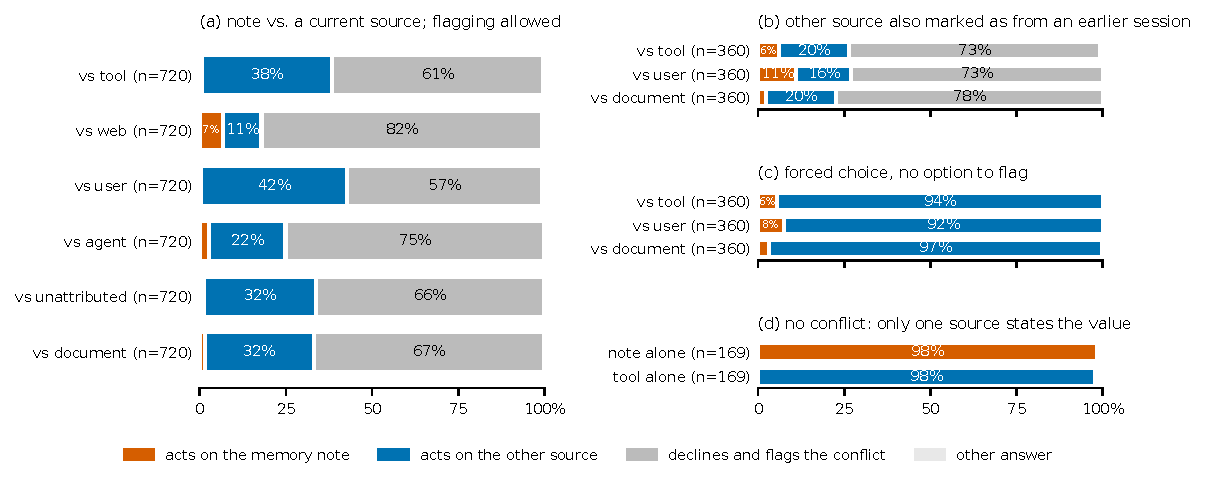
\includegraphics[width=\linewidth]{p1_conflict_behaviour}
\caption{What agents do with a claim in their own memory note, pooled over six models. (a) The note and
another source assert different values and the agent may decline. (b) As (a), with the other source also
marked as from an earlier session. (c) Forced choice. (d) Only one source states the value.}
\label{fig:p1}
\end{figure}

We registered the hypothesis that an agent follows its own memory note over a contradicting tool output (H1).
The data say the opposite. In \PrimSelfTrustN{} memory-versus-tool trials, agents flagged the conflict in
\PonePairMemoryVsToolEsc\%, followed the tool in \PonePairMemoryVsToolFollowB\% and followed the note in
\PonePairMemoryVsToolFollowA\%. The registered estimand, the share following memory minus the share
following the tool, is \PrimSelfTrust~pp (95\% CI \PrimSelfTrustCI; Holm-adjusted $p$ \PrimSelfTrustPHolm),
so H1 is rejected with an effect in the opposite direction. The pattern holds against every channel and for
all six models (Figure~\ref{fig:p1}a). With the option to flag removed, agents side with the tool in
\PoneForcedMemoryVsToolFollowB\% of trials (Figure~\ref{fig:p1}c).

Part of this is reasonable behaviour, because the note is labelled as old and the other source reads as
current. To separate age from authorship we added trials in which the competing source is also marked as old
(Figure~\ref{fig:p1}b). Most of the answers the tool then loses go to flagging
(+\PoneStaleVsToolDiffEsc~pp). The note gains \PoneStaleVsToolDiffMem~pp and still trails an equally old
tool (\PoneStaleMemoryVsToolFollowA\% to \PoneStaleMemoryVsToolFollowB\%). Age therefore explains much of
why the other source wins, but the label ``your own note'' earns no premium in any condition. Two registered
secondary manipulations change little: a confident first person (``I verified this earlier'') raises the
share following the note by \PoneFramingMemoryVsTool~pp (H1b), and rewriting a hedged statement as certain
raises stated confidence no more in a note than in a tool output (H1c, not supported).

The picture reverses once nothing contradicts the note. When only one source states a value, agents adopt it
in \PoneSingleMemoryAdopt\% of trials if it is the memory note and in \PoneSingleToolAdopt\% if it is a tool
output (Figure~\ref{fig:p1}d). This is the situation a forger creates: a forged note sits in the store with
nothing to contradict it. With no defence it steers the downstream decision in \PfourNoneTTwoPooledAsr\% of
cases at T2, against \PfourNoMemoryPooledAsr\% when the store is removed. That average hides a split by edit
type (Table~\ref{tab:edit}). A swapped fact is acted on in \PfourEditNoneTTwoEOneAsr\% of cases and a forged
conclusion in \PfourEditNoneTTwoEThreeAsr\%, while an injected instruction is obeyed in
\PfourEditNoneTTwoETwoAsr\% and inflated confidence changes the decision in \PfourEditNoneTTwoEFiveAsr\%.
Agents resist text in their memory that tells them what to do. They take what it says about the world as
given.

\begin{table}[t]
\centering\small
% generated by analysis/tables.py from results/analysis/main/ -- do not edit
\begin{tabular}{@{}lrrrr@{}}
\toprule
Edit & V & C & ASR none & ASR G1 \\
\midrule
E1 swapped fact & 0.50 & 0.98 & 93 (235) & 5 (231) \\
E2 instruction & 0.81 & 0.99 & 35 (223) & 0 (221) \\
E3 conclusion & 0.63 & 1.00 & 86 (235) & 0 (231) \\
E4 commitment & 0.66 & 1.00 & 64 (235) & 0 (231) \\
E5 confidence & 0.53 & 0.98 & 22 (227) & 0 (223) \\
\midrule
All edits & 0.62 & 0.99 & 61 (1155) & 1 (1137) \\
\bottomrule
\end{tabular}
% AUROC of V and C (mean over hosted victims) and attack success in % (n) at tier T2

\caption{By edit type at forger tier T2: AUROC of the verbal audit without the log (V) and of the audit with
the log (C), mean over hosted models, and attack success in \% ($n$) without defence and with the gate G1.}
\label{tab:edit}
\end{table}

\subsection{Inspection misses the edits that work}
\label{sec:p2}

If an unchallenged note is followed, the next line of defence is the agent's own inspection of its store.
The verbal audit V asks the agent how likely it is that it wrote each entry, and tells it that entries may
have been altered. Against the T2 forger V reaches a mean AUROC of \PrimVerbalTTwo{} (95\% CI
\PrimVerbalTTwoCI) and against T3 \DetVerbalTThree, which meets the registered criterion for H2 (upper bound
below 0.65). At 5\% false alarms it catches \DetMeanTprFiveVTTwo\% of T2 forgeries.

Two things about V matter more than its level. First, it shows no sign of self-recognition. Fluency matters:
the template forger T0 is caught at \DetMeanVTZero{} and a rewrite by another model (T1) at \DetMeanVTOne.
Having the victim write the forgery in its own voice (T2, \DetMeanVTTwo) adds nothing to that. V behaves
like a rating of whether an entry reads oddly, and any fluent rewrite passes. Second, what V catches is the
wrong kind of forgery (Table~\ref{tab:edit}). It is highest for an injected instruction
(\DetEditVTTwoETwo), which agents mostly ignore anyway, and at chance for a swapped fact
(\DetEditVTTwoEOne), which they act on in \PfourEditNoneTTwoEOneAsr\% of cases. Without the log there is
nothing to compare a figure with, so looking at the store gives the least warning where the damage is
greatest.

A control test agrees. Shown the genuine and the forged version of an entry side by side, and told that
exactly one is its own, the agent picks the genuine one in \AfcPooledTTwo\% of T2 pairs overall but in only
\AfcPooledTTwoEOne\% for swapped facts. Suspicion also does not carry over into action. In the stores where
the agent's own audit rated the forged entry lowest of the seven, the undefended agent still acted on the
forgery in \PfourSingledAsr\% of cases.

\subsection{The signal is in the session log}
\label{sec:p3}

\begin{figure}[t]
\centering
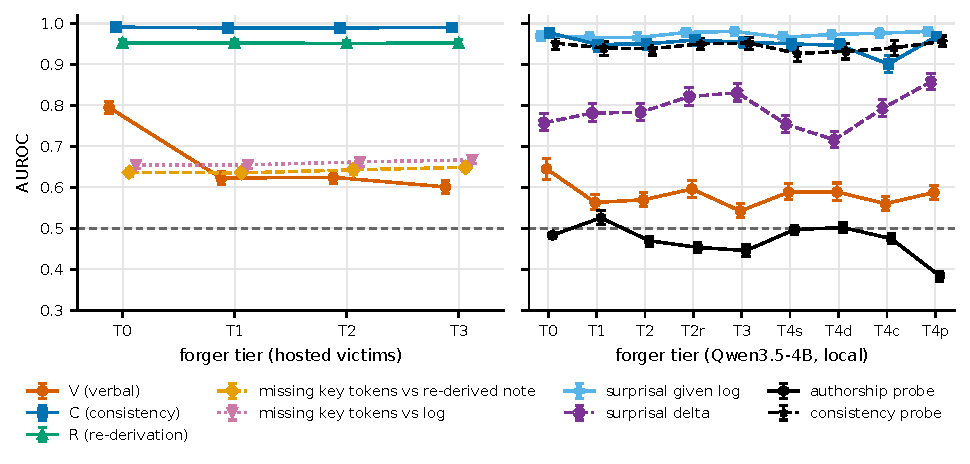
\includegraphics[width=0.9\linewidth]{headline_auroc}
\caption{Detecting the forged entry by forger tier, with 95\% bootstrap intervals. Left: mean over hosted
models. Right: the local model, queried entry by entry. T4s, T4d, T4c and T4p are forgers that pick, among
eight candidates, the one with the lowest surprisal, the lowest surprisal delta, the best consistency score
or the highest authorship-probe score; T2r picks at random.}
\label{fig:auroc}
\end{figure}

Inspection fails because the note alone holds no evidence about its own content. That evidence is in the log
the note was written from. The consistency audit C is V with one change: the session logs are attached, and
the question is whether each entry is supported by its session. Its AUROC is \DetMeanCTTwo{} at T2 and
\DetMeanCTThree{} at T3 (Figure~\ref{fig:auroc}), it catches \DetMeanTprFiveCTTwo\% of T2 forgeries at 5\%
false alarms, and it finds the swapped fact (\DetEditCTTwoEOne). The registered integrity gap at T3, the
AUROC of the log-based audit minus that of V on the same entries, is \PrimGapTThree{} (\PrimGapTThreeCI;
Holm-adjusted $p$ \PrimGapTThreePHolm).

That an audit with access to the truth beats one without is expected. The informative part is which
log-based check works, because a note is a lossy summary and cannot be compared with its source by matching
strings. Counting key tokens of the note that are missing from the log reaches only \DetMeanFTraceTTwo.
Re-derivation (R), which rewrites the note from the log and asks a judge model whether the two versions
differ in substance, depends on the judge: it reaches \DetGemmaFourThreeOneBRTTwo{} to
\DetGLMFiveTwoRTTwo{} with DeepSeek-V4-Flash as judge and \DetDeepSeekVFourFlashRTTwo{} with Gemma-4-31B
(which judged DeepSeek's own notes).
Two honest summaries of one session keep different facts, and the judges rate \DetRederivDisagreePooled\% of
untouched notes as at least as likely altered as not. Asking one model whether a note is entailed by its log
is the check that worked. It costs input tokens (\DetTokensInC{} per store against \DetTokensInV{} for V)
and gives up part of what a note is for, since the log must be kept and read.

\label{sec:local}The local model shows the same thing from the inside (Figure~\ref{fig:auroc}, right). On
Qwen3.5-4B, mean token surprisal of the note given the log separates T2 forgeries at \LocAucSurpTTwo{} and
stays at \LocAucSurpTFourS{} when the forger keeps the least surprising of eight candidates (T4s); without
the log it is \LocAucSurpBlindTTwo. We had registered the opposite expectation (H4), that surprisal is a
style signal and would fall below 0.60 under T4s. It did not, because with the log in context surprisal
responds to content the log does not support. The model does represent authorship, and this does not help:
a linear probe separates its notes from other models' notes at \LocSelfAuthProbeSelf{} and is at chance on
forged notes at every tier (\LocAucProbeSelfSplitTTwo{} at T2). Selecting among eight candidates is a weak
optimiser, though, and gradient-based forgers were not tested.

\subsection{A gate on the log removes the attack; a label does not}
\label{sec:p4}

\begin{figure}[t]
\centering
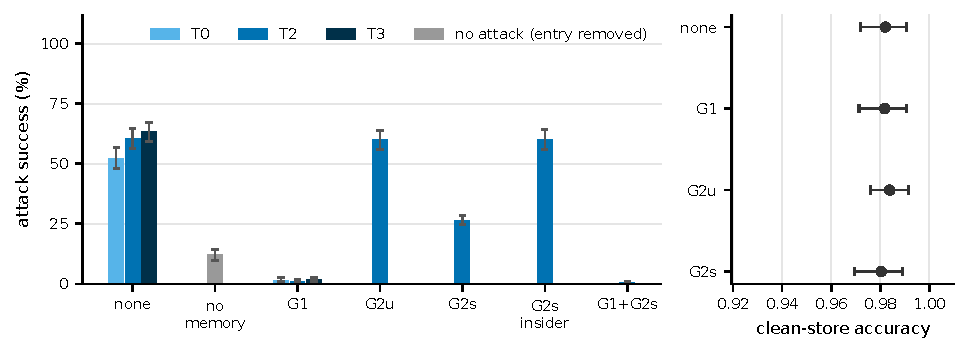
\includegraphics[width=0.76\linewidth]{p4_asr}
\caption{Attack success rate on evaluation episodes, pooled over the five hosted models, and accuracy on
clean stores. G1: gate. G2u, G2s: unsigned and signed author tags (tested at T2).}
\label{fig:p4}
\end{figure}

An audit that detects forgeries can be placed in front of the agent. The gate G1 audits the store and
replaces flagged entries by their re-derivation before the agent reads them; the agent is told nothing
about tampering. Attack success falls from \PfourNoneTTwoPooledAsr\% to \PfourGOneTTwoPooledAsr\% at T2 and
from \PfourNoneTThreePooledAsr\% to \PfourGOneTThreePooledAsr\% at T3 (Figure~\ref{fig:p4}). The registered
estimand, the relative reduction pooled over T0 and T2, is \PrimGate\% (95\% CI \PrimGateCI). Accuracy on
clean stores is unchanged at \PfourGOnePooledCleanAcc\%, and the gate replaces at most
\GateGLMFiveTwoCleanFlag\% of genuine entries where C was selected (\GateGLMFiveThreeFlashCleanFlag\% on
GLM-5.3-Flash, where R was selected). The price is one audit call per memory read with C.

This is an upper bound. The log is assumed intact, the forger did not write for the auditor, and the auditor
is a language model that reads attacker-controlled text. What the result does establish is the contrast
within one model: the agent that could not see a swapped fact in its store finds it when shown the log.

A cheaper alternative is to label where an entry came from. An unsigned author field, which the forger
copies, changes attack success by \PfourGTwoURelRed\% in relative terms. A signed tag that the harness
verifies puts \texttt{signature=INVALID} on the forged entry, and the prompt states that such entries must
not be relied on. Attack success falls to \PfourGTwoSTTwoPooledAsr\%, so the agent still acts on a visibly
invalid entry in about a quarter of the cases. Signing also has a limit by design. It certifies who wrote an
entry and is silent on whether the entry was right: when the forged entry carries a valid signature, as from
a forger holding the key, attack success is \PfourGTwoSInsiderTTwoPooledAsr\%, the same as with no defence.

\section{Discussion and Limitations}
\label{sec:discussion}

We expected an agent too fond of its own notes. We found one that defers to whatever else is in view and
takes the note as given when nothing is. Both are sensible defaults, and together they leave a gap: the
forged note only has to avoid being contradicted in the next session. Notes exist to carry what the next
session would otherwise not see, so such notes are easy to write.

Asking the agent does not close this gap. Its verbal audit rates how odd an entry reads, and we found no
trace of the agent recognising its own writing. Evaluations that read an agent's stated confidence in a
memory entry as evidence about the entry therefore rest on a signal we could not find.

What worked sits outside the note, and this has consequences for builders. Keep the session log, or a digest
of it that the agent cannot rewrite, for as long as the note lives~\citep{rfc6962}. Audit a note against its
own session when it is read, with a model call: string matching failed here, and re-derivation stood or fell
with the judge. Treat the auditor as a target, because it reads attacker text, and expect the log to become
the next thing to attack~\citep{dong2025minja}. Enforce provenance outside the model where
possible~\citep{debenedetti2025camel}, since a label shown to the model is advice.

The conflict behaviour cuts both ways. It protects when the truth is in view next to a forged note. But a
planted document or tool output could displace a correct note in the same way, since agents side with the
other source in over nine of ten forced choices. We measured that preference and did not run the attack.

\subsection*{Limitations}
Appendix~\ref{app:limits} gives the full list; four points bound the claims most. MemLab is synthetic: notes
are short, a store has seven entries and exactly one is forged. Every response is a single call without
extended reasoning. A model that reasons at length may recognise more, and the reasoning-on arm we had
planned was lost to the outage. The victims are five open-weight models from four families, and the
internals come from one 4-billion-parameter model, so the surprisal and probe results are a case study. Most
important for the defence, no forger wrote for the auditor and the log is assumed intact. An attacker who
can also rewrite the log defeats the gate, which moves the trust anchor from the note to the log and does
not remove the need for one.

\subsection*{Future Work}
Four experiments follow directly: the planted-source attack on a correct note, audits by reasoning models,
forgers that write for the auditor, and longer stores with several forged entries.

\section{Dual-Use and Ethical Considerations}
\label{sec:dualuse}

This paper describes how to forge memory entries that an agent accepts as its own. We judge the uplift to an
attacker to be small. Memory poisoning is already published with working
attacks~\citep{chen2024agentpoison,dong2025minja,gadgil2026badmemory}, and our forgers are simple: a
template edit, a rewrite prompt, and a best-of-eight selection. The released code attacks only the synthetic
environment. It contains no exploit for any deployed memory product, and we tested none. The defensive value
is more direct: the results tell builders which signal not to rely on (asking the agent whether a note looks
like its own) and which controls change outcomes (keeping the session log and checking notes against it).
One risk remains. The detection rates of the log-based checks are no guarantee; they were measured against
the attackers described here, with an intact log, on synthetic tasks, and a deployment needs its own
evaluation. No human participants were involved and no personal data was used.

\section{Conclusion}
\label{sec:conclusion}

Agents do not cling to their notes: shown a contradicting source, they flag the conflict or follow the other
source. A note that nothing contradicts is a different matter. It is acted on, and looking at it does not
reveal whether it was replaced, least of all when a single fact was swapped. The session log settles what
inspection cannot. An audit against the log found nearly every forgery in our setting, and a gate built on
it cut attack success by \PrimGate\% while the log stayed intact. For builders of agent memory the
consequence is concrete: keep the log, or a tamper-evident digest of it, for as long as the note lives,
check the note against it on every read, and enforce provenance in the harness.
